%
% CMPT 300: Operating Systems I - A Course Overview
% Section: Scheduling
%
% Author: Jeffrey Leung
%

\section{Scheduling}
	\label{sec:scheduling}
\begin{easylist}

& Process execution switches between bursts of CPU execution and I/O wait
	&& \textbf{I/O bound process:} Process which spends more time in I/O waits than CPU execution
	&& \textbf{CPU bound process:} Process which spends more time in CPU execution than I/O waits

& %TODO diagram

& \textbf{Long-term/job scheduler:} Component which decides which processes should be moved to the ready queue, to maintain a balanced mix of I/O-bound and CPU-bound processes
	&& Controls degree of concurrency/multiprogramming
	&& Slow; invoked infrequently
& \textbf{Midterm scheduler:} Component which holds partially-executed processes which are not in the ready queue %TODO

& \textbf{Short-term/CPU scheduler:} Component which decides which processes from the ready queue the CPU should perform work for
	&& Quick; invoked frequently (every several milliseconds)
	&& \textbf{Nonpreemptive:} Process which can only stop during CPU execution by terminating or by waiting (e.g. I/O request, child termination)
	&& \textbf{Preemptive:} Process which can be forcefully stopped (preempted) during CPU execution by the OS (e.g. to run a higher-level process)
		&&& More difficult to implement
			&&&& Needs to maintain consistency of data shared between processes and kernel data structures (e.g. I/O queues)
			&&&& Needs hardware support (e.g. timers)

& \textbf{Dispatcher:} Component which allocates the CPU to various processes by switching context, switching user mode, jumping to the specified location in the process, and restarting execution
	&& \textbf{Dispatch latency:} Time required for the dispatcher to switch tasks

\end{easylist}
\subsection{Scheduling Algorithms}
	\label{subsec:scheduling:algorithms}
\begin{easylist}


& Criteria:
	&& Maximize CPU utilization
	&& Maximize throughput
	&& Minimize first response time
	&& Minimize waiting time (time before a process starts exeuction)
	&& Minimize job turnaround time

& \textbf{Convoy effect:} Suboptimal situation where a long process blocks the CPU, requiring shorter processes to wait
	&& Utilization of CPU and device is low

& \textbf{First-Come, First-Served (FCFS):} CPU scheduling algorithm which prioritizes processes based on when they are placed in the queue
	&& Tasks which take longer will block other tasks; a CPU-bound process would block I/O-bound processes
	&& Examples:
		&&& For tasks P\textsubscript{1} = 24ms, P\textsubscript{2} = 3ms, P\textsubscript{3} = 3ms in the given order (see diagram~\ref{fig:scheduling:gantt-1}), the average waiting time is $\frac{0 + 24 + 27}{3} = 17 \text{ms}$
		
\begin{figure}[!htb]
	\centering
	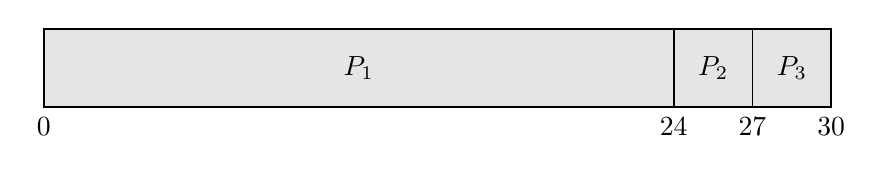
\begin{tikzpicture}[line width=.7pt]
		\draw[fill=gray!20] (0,0)node[below]{0} rectangle(8,1);
		\draw[fill=gray!20] (8,0)node[below]{24} rectangle(9,1);
		\draw[fill=gray!20] (9,0)node[below]{27} rectangle (10,1) node[below,yshift=-1cm]{30};
		\path (4,0.5) node{$P_1$} (8.5,0.5) node{$P_2$} (9.5,0.5) node{$P_3$};
	\end{tikzpicture}
	\caption{FCFS Gantt Chart for P\textsubscript{1} = 24ms, P\textsubscript{2} = 3ms, P\textsubscript{3} = 3ms}
	\label{fig:scheduling:gantt-1}
\end{figure}

		&&& For tasks P\textsubscript{2} = 3ms, P\textsubscript{3} = 3ms, P\textsubscript{1} = 24ms in the given order, the average waiting time is $\frac{0 + 3 + 6}{3} = 3 \text{ms}$


& \textbf{Shortest Job First (SJF):} CPU scheduling algorithm which prioritizes processes based on shortest execution time (without preempting currently running processes)
	&& Provably optimal in giving minimum average waiting time for a given set of processes
	&& Length of next CPU burst is available for long-term scheduling but not available for short-term scheduling
	&& Time of execution is approximated through prediction from previous executions %TODO
	&& Examples:
		&&& For tasks: %TODO
	&&& Time prediction %TODO
& \textbf{Shortest Remaining Time First (SRTF):} CPU scheduling algorithm which prioritizes processes based on the least execution time remaining, switching between processes when necessary
	&& Examples: %TODO
& \textbf{Round Robin:} CPU scheduling algorithm which provides a unit of time (\textit{q)}) for each process before moving to the next process
	&& \textbf{Time quantum} ($q$): Unit of CPU time (10-100 ms) for which a process can execute
		&&& For $n$ processes in the ready queue, each process receives $\frac{1}{n}$ of CPU time
		&&& $q$ and context switch time %TODO
	&& Process is moved to end of (circular) ready queue once its time is finished
	&& Better response time and higher average turnaround time (vs. SJF)

& \textbf{Priority scheduling:} CPU process scheduling which allocates work depending on a priority level
	&& SJF is when the priority is the inverse of the CPU burst length
	&& \textbf{Starvation:} Failure to allocate a low-priority process
		&& \textbf{Aging:} %TODO

& \textbf{Multilevel queue scheduling:} Scheduling design with multiple prioritized ready queues, each with its own scheduling algorithm
	&& %TODO

& \textbf{Multiprocessor scheduling:}
	&& Divide load among multiple processors
	&& \textbf{Asymmetric multiprocessor:} Multiprocessor scheduling strategy where one master processor handles all scheduling
	&& \textbf{Symmetric multiprocessor:} Multiprocessor scheduling strategy where %TODO
		&&& Issues:
			&&&& \textbf{Processor affinity:} Binding and unbinding of a process to the CPU
				&&&&& When a process is migrated to a new processor, the old cache must be invalidated and the new cache must be re-populated which has a performance penalty
			&&&& \textbf{Load balancing:} Workload distribution among various processors
				&&&&& \textbf{Push migration:} Task repeatedly checks all processors and moves tasks to evenly distribute them
				&&&&& \textbf{Pull migration:} Idle processor taking a task from a busy processor
			&&&& Tradeoff between processor affinity and load balancing

& \textbf{Real-time scheduling:} %TODO

& \textbf{Completely Fair Scheduler:} %TODO
	&& \textbf{Target latency:} Duration of time during which every runnable task should be executed at least once
		&&& \textbf{Nice value:} Duration of time during which... %TODO

& How algorithms are designed:
	&& Use deterministic modelling to run algorithms on workloads
	&& Use queuing models and theory to analyze algorithms (using typically unrealistic assumptions)
	&& Use a simulator to model systems (using a synthetic workload or traces from real systems)
		&&& Expensive and time-consuming

\end{easylist}
\clearpage